\runningheader{Oppgave b)}{}{Side \thepage\ av \numpages}
% ********************************************************
% oppgave b) 
% ********************************************************  
\item
{\bf Numerisk integrasjon og derivasjon i Matlab}
\label{oppg:b}

I denne oppgaven skal du ta
utgangspunkt   i skallfilen \fbox{\tt oving3\_skallfil.m} for å  
lage kode for numerisk
integrasjon av
$u(t)$ fra ligning~\eqref{eq:u} ved å bruke både {\it Eulers  forovermetode},
  {\it  Eulers  bakovermetode} og {\it  trapes\-metoden}, henholdsvis gitt som:
  \begin{alignat}{3}
    &y_{k} && =  y_{k-1} +
              T_s {\cdot} u_{k-1}, 
    &&~~ \forall ~  k{=}2,\ldots,n \quad \text{gitt } y_{1} \label{eq:ef}\\
    &y_{k} && =  y_{k-1} +
              T_s {\cdot} u_{k}, 
    &&~~\forall ~  k{=}2,\ldots,n\quad \text{gitt } y_{1} \label{eq:eb}\\
    &y_{k} && =  y_{k-1} +
              T_s {\cdot} \frac{1}{2}{\cdot} \bigl(u_{k-1} + u_{k} \bigr),
    &&~~\forall ~  k{=}2,\ldots,n \quad \text{gitt } y_{1} \label{eq:tr}
  \end{alignat}
  
  
  Du skal også utføre kodebasert numerisk derivasjon   av
$u(t)$ ved å bruke både {\it bakoverderivasjon}, 
  {\it  foroverderivasjon}, 
  og {\it  senter\-derivasjon}, henholdsvis  gitt som 
  \begin{alignat}{3}
    & v_{k} && =\frac{u_{k}-u_{k-1}}{T_s}, &&\quad  \forall ~
            k{=}2,\ldots,n \quad \text{gitt } v_{1}=0 \label{eq:bak}\\
    & v_{k-1} && =\frac{u_{k}-u_{k-1}}{T_s},&&\quad\forall ~ k{=}2,\ldots,n\\
    & v_{k-1} && =\frac{u_{k}-u_{k-2}}{2{\cdot}T_s}, &&\quad\forall ~
              k{=}3,\ldots,n \quad \text{gitt } v_{1}=0
  \end{alignat}
   
  \begin{itemize}
  \item Ferdigstill den uferdige koden for denne deloppgaven, og
    vis at du får følgende resultat (ta med din egen figur
    i innleveringen).
    \begin{figure}[H]
      \centering
      \hspace*{10mm}\scalebox{0.45}{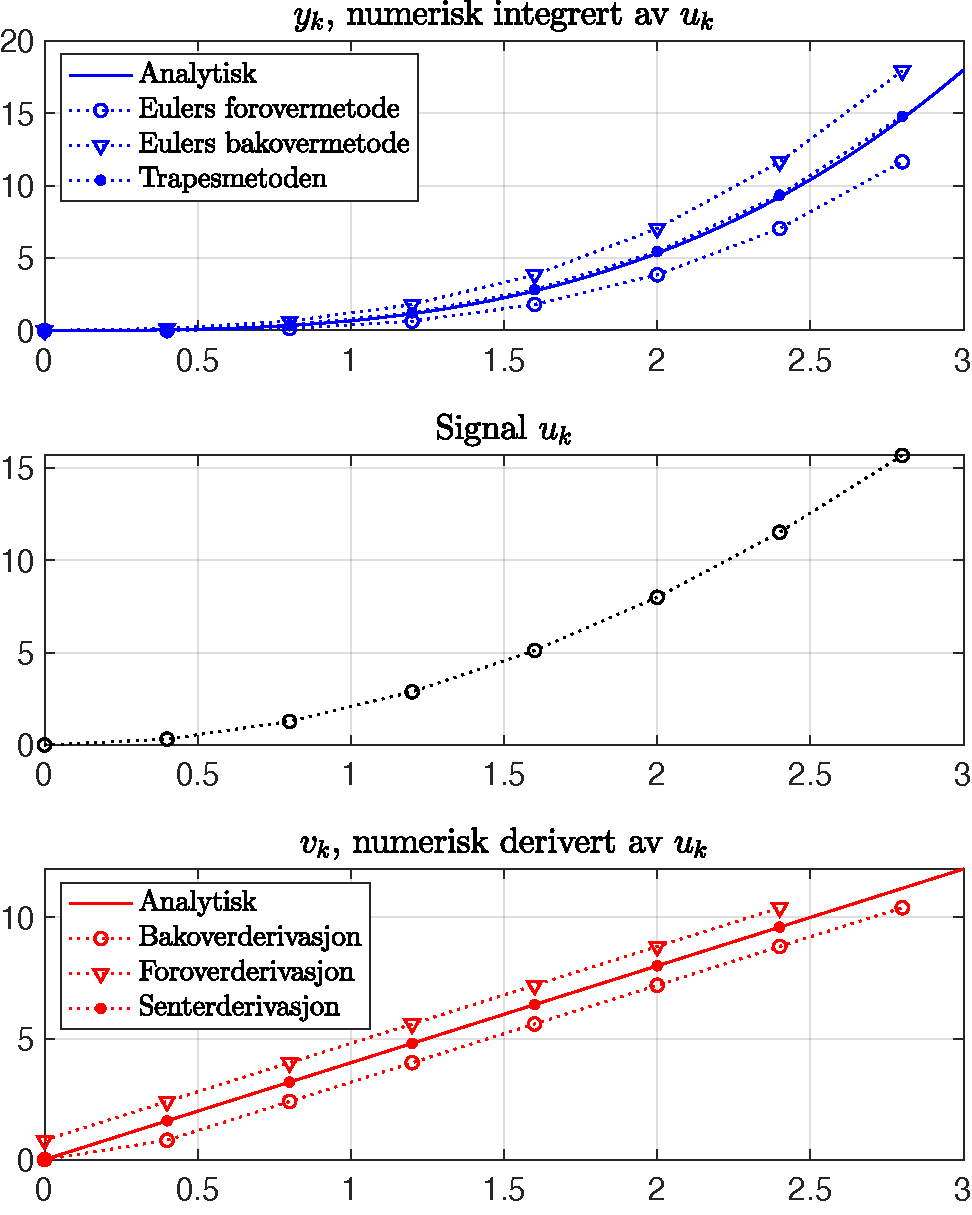
\includegraphics{fig3b_1.pdf}}
      \caption{Simuleringsresultat }
      \label{fig:fig3b_1}
    \end{figure}


  Når du skal plotte forover- og senterderivasjon,
  så må du passe på at dimensjonene til tidsvektoren og henholdsvis
  {\tt  v\_forover(k)} og  {\tt v\_senter(k)} er like lange. 
  
\item
  Avles verdiene av  {\tt y\_EulerF(k)},  {\tt y\_EulerB(k)} og
  {\tt y\_Trapes(k)} ved tidspunkt $t_{k}{=}2$~sekund som i
  deloppgave~\ref{oppg:a}), og vis at de er identiske med
  {\color{blue}\fbox{$y_{k}$}}-verdiene du fant der.

\item
  Avles verdien av  {\tt v\_bakover(k)} 
  ved tidspunkt $t_{k}{=}2$~sekund som i
  deloppgave~\ref{oppg:a}), og vis at den er identiske med
 alle tre {\color{red}\fbox{$v_{k}$}}-verdiene du fant der. 
  \end{itemize}

